\section{问题二：基于 YOLOv8 的缺陷检测模型}

\subsection{YOLOv8 检测模型}

YOLOv8 是 Ultralytics 提出的单阶段目标检测框架\cite{jocher2023}，采用 anchor-free 解耦检测头设计，整体由 Backbone、Neck 与 Head 三部分组成，其结构示意如图 \ref{fig:yolo} 所示。Backbone 以 C2f 模块堆叠提取多尺度特征，并经 SPPF 池化增强感受野；Neck 采用 PAN-FPN 结构实现自顶向下与自底向上的双向多尺度特征融合，输出 P3、P4、P5 三组特征图；Head 对每个位置直接预测类别与包围框（anchor-free），并通过解耦分支分别进行回归与分类，最后经非极大值抑制（NMS）输出检测结果。

\begin{figure}[H]
\centering
\resizebox{\textwidth}{!}{%
\begin{tikzpicture}[
  node distance=0.5cm and 0.45cm,
  every node/.style={font=\zihao{-5}},
]
  \node[figbox] (in) {输入图像\\$640\times640\times3$};
  \node[corebox, right=of in] (bb) {Backbone\\Conv + C2f + SPPF};
  \node[altbox, right=of bb] (nk) {Neck\\PAN-FPN 双向融合\\P3/P4/P5};
  \node[corebox, right=of nk] (hd) {解耦检测头\\P3/P4/P5};
  \node[corebox, right=of hd] (nm) {NMS\\后处理};
  \node[outbox, right=of nm] (out) {输出\\位置+类别+置信度};

  \node[altbox, below left=0.55cm and 0.2cm of hd] (cls) {分类分支\\$C$ 类置信度};
  \node[altbox, below right=0.55cm and 0.2cm of hd] (reg) {回归分支\\$4$ 维框坐标 + DFL};

  \node[stagetitle, above=0.12cm of bb] {Backbone};
  \node[stagetitlealt, above=0.12cm of nk] {Neck};
  \node[stagetitle, above=0.12cm of hd] {Head};

  \draw[figarr] (in) -- (bb);
  \draw[figarr] (bb) -- (nk);
  \draw[figarr] (nk) -- (hd);
  \draw[figarr] (hd) -- (nm);
  \draw[figarr] (nm) -- (out);
  \draw[figarr] (hd) -- (cls);
  \draw[figarr] (hd) -- (reg);
\end{tikzpicture}}
\caption{YOLOv8 网络结构示意图}\label{fig:yolo}
\end{figure}

YOLOv8 的总体训练损失由定位损失、分类损失与分布聚焦损失三部分加权组成：
\begin{equation}
  \mathcal{L} = \lambda_{\mathrm{box}}\mathcal{L}_{\mathrm{box}}
              + \lambda_{\mathrm{cls}}\mathcal{L}_{\mathrm{cls}}
              + \lambda_{\mathrm{dfl}}\mathcal{L}_{\mathrm{dfl}},
  \label{eq:total_loss}
\end{equation}
其中定位损失采用 CIoU 损失。对预测框 $B$ 与真实框 $B^{\mathrm{gt}}$，记两者交集与并集的面积分别为 $|B\cap B^{\mathrm{gt}}|$ 与 $|B\cup B^{\mathrm{gt}}|$，则
\begin{equation}
  \mathrm{IoU} = \frac{|B\cap B^{\mathrm{gt}}|}{|B\cup B^{\mathrm{gt}}|},
  \label{eq:iou}
\end{equation}
\begin{equation}
  \mathcal{L}_{\mathrm{CIoU}} = 1 - \mathrm{IoU}
  + \frac{\rho^{2}(\bm{b},\bm{b}^{\mathrm{gt}})}{c^{2}} + \alpha v,
  \label{eq:ciou}
\end{equation}
其中 $\rho(\cdot)$ 为两框中心点的欧氏距离，$c$ 为最小外接矩形对角线长度，$\alpha$ 为平衡系数，$v$ 度量长宽比一致性。分类损失采用二元交叉熵：
\begin{equation}
  \mathcal{L}_{\mathrm{cls}} = -\bigl[y\log\sigma(z) + (1-y)\log(1-\sigma(z))\bigr],
  \label{eq:bce}
\end{equation}
分布聚焦损失以离散分布形式建模边框位置的概率分布\cite{li2020gfl}，并通过
\begin{equation}
  \mathcal{L}_{\mathrm{DFL}}(S_i,S_{i+1}) = -\bigl[(y_{i+1}-y)\log S_i + (y-y_i)\log S_{i+1}\bigr]
  \label{eq:dfl}
\end{equation}
引导预测分布向真实位置集中，其中 $y_i,y_{i+1}$ 为真实位置的相邻整数值，$S_i,S_{i+1}$ 为对应的预测概率。

\subsection{训练策略与实验设置}

本文全部实验基于 PyTorch 与 Ultralytics 框架，在固定随机种子（seed=42）下进行，保证结果可复现。实验环境与统一超参数如表 \ref{tab:setup} 所示。

\begin{table}[H]
\centering
\zihao{5}
\caption{实验环境与统一训练超参数}\label{tab:setup}
\begin{tabular}{llll}
  \toprule
  类别 & 配置 & 类别 & 配置 \\
  \midrule
  GPU & RTX 4070 Laptop（8 GB） & 输入尺寸 & $640\times640$ \\
  Python & 3.13 & 批大小 & 16 \\
  PyTorch & 2.13 & 初始学习率 lr0 & 0.01 \\
  Ultralytics & 8.4.110 & 学习率衰减 lrf & 0.01，余弦退火 \\
  优化器 & SGD（momentum=0.937） & 权重衰减 & $5\times10^{-4}$ \\
  热身轮数 & 3 & 早停耐心 & 20 \\
  混合精度 & AMP & 随机种子 & 42 \\
  \bottomrule
\end{tabular}
\end{table}

本文设计三组递进对照实验，配置如表 \ref{tab:exps} 所示：基线实验用于建立基准；改进实验升级骨干网络并引入 Copy-Paste 增强；最终模型进一步加入 600 幅负样本参与训练，用于问题一判别与背景误检抑制。

\begin{table}[H]
\centering
\zihao{5}
\caption{三组实验配置}\label{tab:exps}
\begin{tabular}{lcccc}
  \toprule
  实验 & 骨干网络 & 训练轮数 & Copy-Paste & 负样本数 \\
  \midrule
  基线 & YOLOv8n（3.01 M 参数） & 100 & 0 & 0 \\
  改进 & YOLOv8s（11.13 M 参数） & 150 & 0.5 & 0 \\
  最终模型 & YOLOv8s（11.13 M 参数） & 150 & 0.5 & 600 \\
  \bottomrule
\end{tabular}
\end{table}

\subsection{改进策略}

\subsubsection{Copy-Paste 数据增强}

针对 Hole 类样本仅占 11.8\% 的类别不平衡问题，本文启用基于实例混合的增强策略（与 MixUp\cite{zhang2018mixup} 同属混合类方法）：Copy-Paste\cite{ghiasi2021} 以概率 $p=0.5$ 从训练批次中随机选取少数类目标实例，将其像素区域及其标注框一并复制粘贴到其他训练图像中，形成新的训练样本。设源图像中实例 $o=(I_o,B_o)$，目标图像为 $I_t$，粘贴变换 $\mathcal{T}$（含随机平移与尺度缩放），则生成样本为
\begin{equation}
  (I', B') = \bigl(I_t \oplus \mathcal{T}(I_o),\ B_t \cup \mathcal{T}(B_o)\bigr),
  \label{eq:copypaste}
\end{equation}
其中 $\oplus$ 表示像素级融合。该增强在不改变真实语义的前提下成倍扩充少数类样本数量，同时保留实例的上下文外观，有效缓解了 Hole 类梯度不足的问题。

\subsubsection{负样本参与训练}

训练集全部为含缺陷图像，直接训练会使检测网络缺乏对“无缺陷背景”的判别经验，导致背景误检，并干扰问题一判别模型的置信度分布。本文从训练图像中不覆盖任何标注框的区域随机裁剪 $320\times320$ 子图，构造 600 幅负样本并入训练集（标注文件为空）。检测网络据此学习抑制背景响应，使无缺陷图像的最大置信度整体下移，为问题一 EVT 判别提供更清晰的分布分离基础。

\subsubsection{损失函数层面的进一步设计：WD-Focal Loss}

为进一步缓解类别不平衡，本文在 Focal Loss\cite{lin2017focal} 基础上设计并实现了基于 Wasserstein 距离的自适应焦点损失（WD-Focal Loss）。其核心思想是以各类别特征分布与全局参考分布之间的 1-Wasserstein 距离 $W_1(\mu_c,\bar{\mu})$ 动态调制类别平衡系数\cite{villani2009}：
\begin{equation}
  \mathcal{L}_{\mathrm{WD\text{-}FL}}(p_t,c) = -\alpha_c (1-p_t)^{\gamma}\log p_t,
  \qquad \alpha_c = \sigma\!\left(\frac{W_1(\mu_c,\bar{\mu})}{\tau}\right),
  \label{eq:wd_focal}
\end{equation}
其中 $\sigma$ 为 sigmoid 函数，$\tau$ 为温度参数。该损失以特征空间的几何可分性替代样本频率的逆比例加权，理论上对长尾分布更鲁棒，其自适应调制机制如图 \ref{fig:wd_focal} 所示。

\begin{figure}[H]
\centering
\resizebox{\textwidth}{!}{%
\begin{tikzpicture}[
  node distance=0.5cm and 0.45cm,
  every node/.style={font=\zihao{-5}},
]
  \node[corebox] (a) {类别特征分布\\$\mu_c$（Dent/Hole/Rusty）};
  \node[altbox, right=of a] (b) {1-Wasserstein 距离\\$W_1(\mu_c,\bar{\mu})$};
  \node[altbox, right=of b] (c) {自适应平衡系数\\$\alpha_c=\sigma(W_1/\tau)$};
  \node[corebox, right=of c] (d) {WD-Focal Loss\\$-\alpha_c(1-p_t)^{\gamma}\log p_t$};
  \node[outbox, right=of d] (e) {反向传播训练};

  \node[figbox, above=0.55cm of b] (ref) {全局参考分布 $\bar{\mu}$};

  \node[stagetitle, above=0.12cm of a] {特征空间};
  \node[stagetitlealt, above=0.12cm of c] {自适应加权};
  \node[stagetitleout, above=0.12cm of e] {训练};

  \draw[figarr] (a) -- (b);
  \draw[figarr] (b) -- (c);
  \draw[figarr] (c) -- (d);
  \draw[figarr] (d) -- (e);
  \draw[figarr, dashed] (ref) -- (b);
\end{tikzpicture}}
\caption{WD-Focal Loss 的自适应调制机制}\label{fig:wd_focal}
\end{figure}

受竞赛时间限制，本文三组对照实验采用 Ultralytics 默认损失实现，WD-Focal Loss 的完整推导、实现与接口见附录 C，作为后续优化的候选方案。

为检验该候选方案的有效性，本文在赛后补充完成了 WD-Focal Loss 的端到端训练验证（同最终模型配置，150 轮）。首版实现中 $\alpha_c$ 无上限，训练后期各类 $W_1$ 距离相对自适应温度增大，$\alpha_c$ 经 sigmoid 饱和至约 1，负样本权重 $(1-\alpha_c)$ 趋近于 0，模型失去背景抑制并在第 60$\sim$70 轮出现性能崩塌（mAP@0.5:0.95 跌至 0.02$\sim$0.03）；对 $\alpha_c$ 施加 $[0.25,0.75]$ 限幅后崩塌消除，但验证集 mAP@0.5:0.95 仅 0.103，仍显著低于基线（0.205）。值得注意的是，WD-Focal 使 Hole/Dent 两类的 mAP@0.5:0.95 比值由基线的 0.64 升至 1.15，说明 Wasserstein 加权确实将更多权重分配给了少数类 Hole，但其对整体检测精度的负效应表明：聚焦调制在检测场景下的损失尺度（分类梯度占比）需要与框架原有损失重新配平，直接替换不可行。该方向的调参空间（$\gamma$、损失尺度、$\alpha$ 限幅范围）留作后续工作。

\subsection{训练过程与结果}

\subsubsection{训练过程}

最终模型的训练曲线如图 \ref{fig:results_curves} 所示。随着训练进行，三类损失（box、cls、dfl）持续下降并在约 120 轮后趋于平稳，验证集 mAP 同步上升后进入平台期，未出现明显过拟合。训练全程约 173 分钟，验证集指标在第 130$\sim$139 轮附近达到最优。

\begin{figure}[H]
\centering
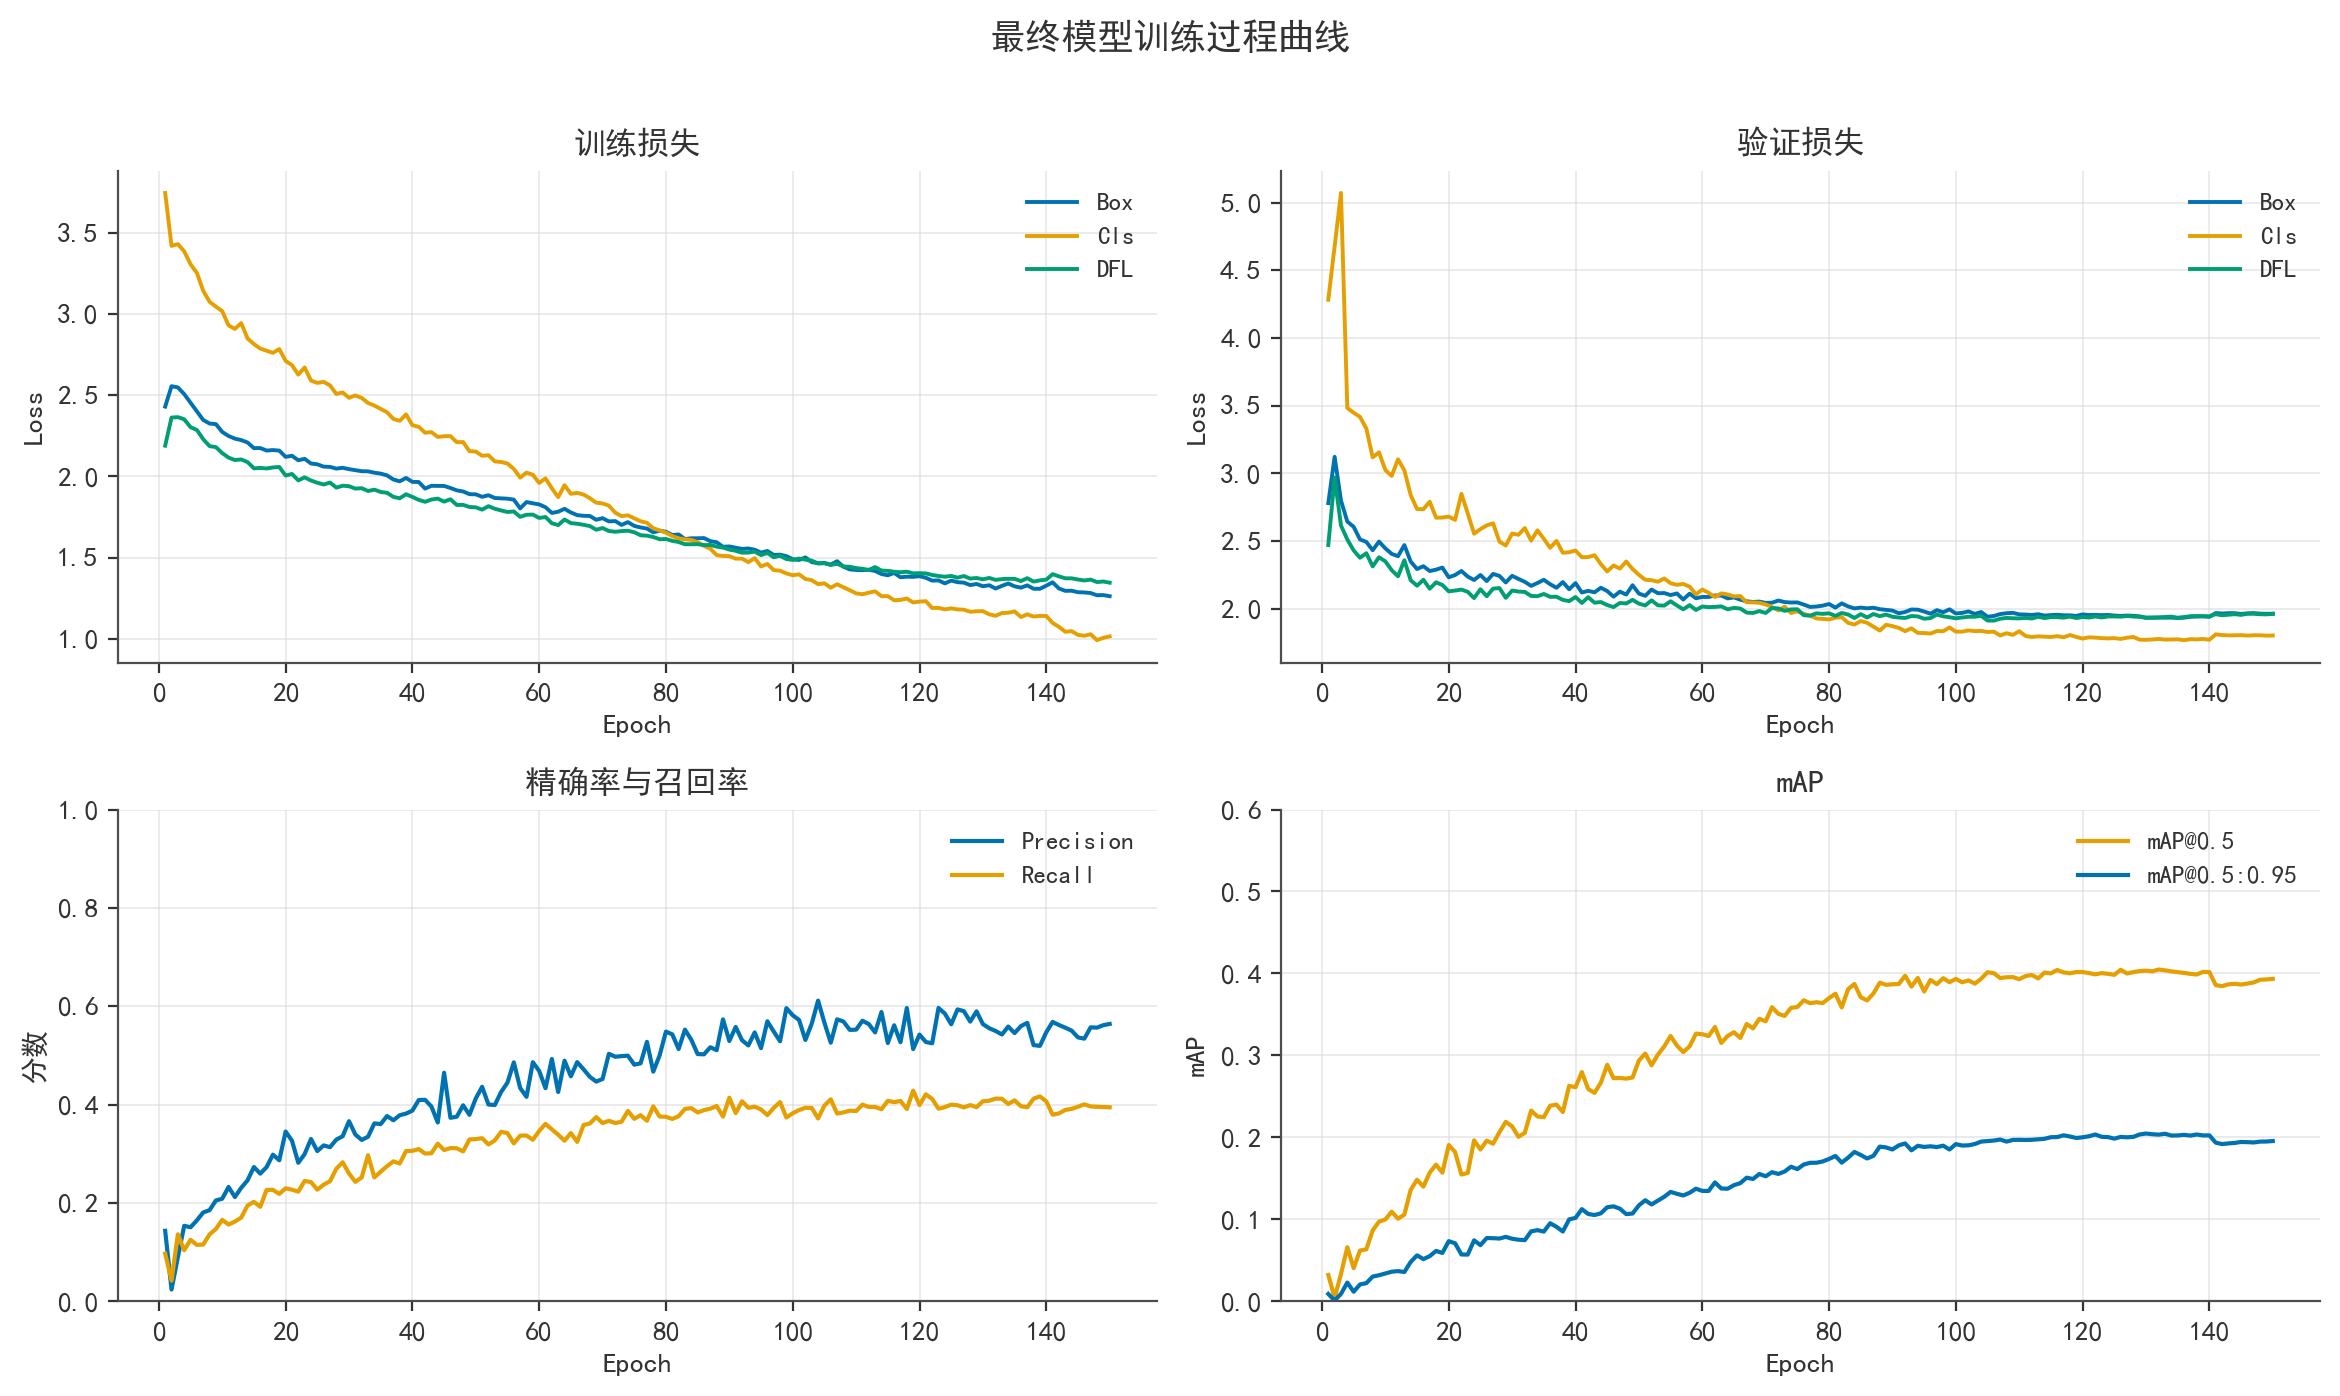
\includegraphics[width=0.98\textwidth]{figures/fig_results_curves.png}
\caption{最终模型训练过程曲线（损失、精确率、召回率与 mAP）}\label{fig:results_curves}
\end{figure}

\subsubsection{三组实验对比}

三组实验在验证集上的最优指标如表 \ref{tab:det_compare} 所示。改进模型相比基线，mAP@0.5 由 0.395 提升至 0.413，mAP@0.5:0.95 由 0.190 提升至 0.212，提升幅度约 11.5\%。为厘清增益来源，本文补充了两组对照：在同配置下将 Copy-Paste 概率分别设为 0 与 0.5 训练，两条 150 轮曲线逐轮完全一致（含训练损失），说明 Copy-Paste 在本数据集（仅目标框标注、无分割掩膜）上未产生可观测增益，上述提升主要来源于骨干网络容量升级（YOLOv8n$\to$YOLOv8s）。最终模型在纯正样本验证集上 mAP 略低于改进模型（mAP@0.5 为 0.405），这是因为负样本训练使模型对低置信度背景响应更加保守，但显著增强了背景抑制能力与问题一判别效果，属于以微小精度代价换取开放集鲁棒性的合理权衡。

\begin{table}[H]
\centering
\zihao{5}
\caption{三组实验验证集最优检测指标对比}\label{tab:det_compare}
\begin{tabular}{lcccc}
  \toprule
  模型 & mAP@0.5 & mAP@0.5:0.95 & Precision & Recall \\
  \midrule
  基线（YOLOv8n） & 0.395 & 0.190 & 0.540 & 0.398 \\
  改进（YOLOv8s+Copy-Paste） & 0.413 & 0.212 & 0.601 & 0.414 \\
  最终模型（+负样本） & 0.405 & 0.205 & 0.550 & 0.412 \\
  \bottomrule
\end{tabular}
\end{table}

\subsubsection{补充消融与改进候选实测}

为进一步量化数据策略与候选改进，本文在赛后补充完成了以下实验（均与最终模型同骨干、同数据、150 轮）：

\begin{enumerate}[leftmargin=2.2em,itemsep=2pt]
  \item {\heiti 负样本数量：}将负样本数分别设为 300、600、900 训练。验证集最优 mAP@0.5:0.95 依次为 0.206、0.205、0.202，差异仅约 0.004；但问题一判别中 Weibull 形状参数 $k$ 依次为 2.879、3.064、2.974，600 幅负样本的置信度分布分离度最高。因此原方案以 600 幅负样本为最终口径同时兼顾检测精度与判别鲁棒性，取舍得到验证；
  \item {\heiti Rusty 类加权：}以 Dent 为基准的逆频率权重（$pos\_weight=3934/3158\approx1.246$）对 Rusty 正样本加权训练，验证集 mAP@0.5:0.95 为 0.171，Rusty 类 mAP@0.5:0.95 由 0.129 略降至 0.114，整体显著下降。该负结果印证了 Rusty 短板来自类间外观混淆而非样本量，单纯损失加权难以弥补；
  \item {\heiti P2 高分辨率检测头：}采用 \texttt{yolov8s-p2}（新增 $160\times160$ 特征图检测头）训练，验证集 mAP@0.5:0.95 为 0.209；Hole 类 mAP@0.5:0.95 由 0.190 升至 0.210、召回率由 0.407 升至 0.453，小目标收益显著，但整体收益有限（+0.005）；
  \item {\heiti 测试时增强（TTA）：}对最终模型启用多尺度测试增强，mAP@0.5:0.95 由 0.204 升至 0.215（+0.011），三类别均提升，且无需重新训练，是性价比最高的改进方向。
\end{enumerate}

\subsubsection{检测结果可视化}

最终模型在验证集上的 PR 曲线与归一化混淆矩阵如图 \ref{fig:pr} 与 \ref{fig:cm} 所示。PR 曲线显示 Dent 类精度-召回权衡最优，Hole 类次之，Rusty 类相对偏弱；混淆矩阵表明主要误检发生在 Rusty 与背景之间。图 \ref{fig:val_labels} 与图 \ref{fig:val_pred} 给出同一批验证图像的标注与预测对比，图 \ref{fig:detect_samples} 给出测试集检测结果示例，模型能够准确定位多类缺陷并输出类别与置信度。

\begin{figure}[H]
\centering
\begin{minipage}[t]{0.48\textwidth}
  \centering
  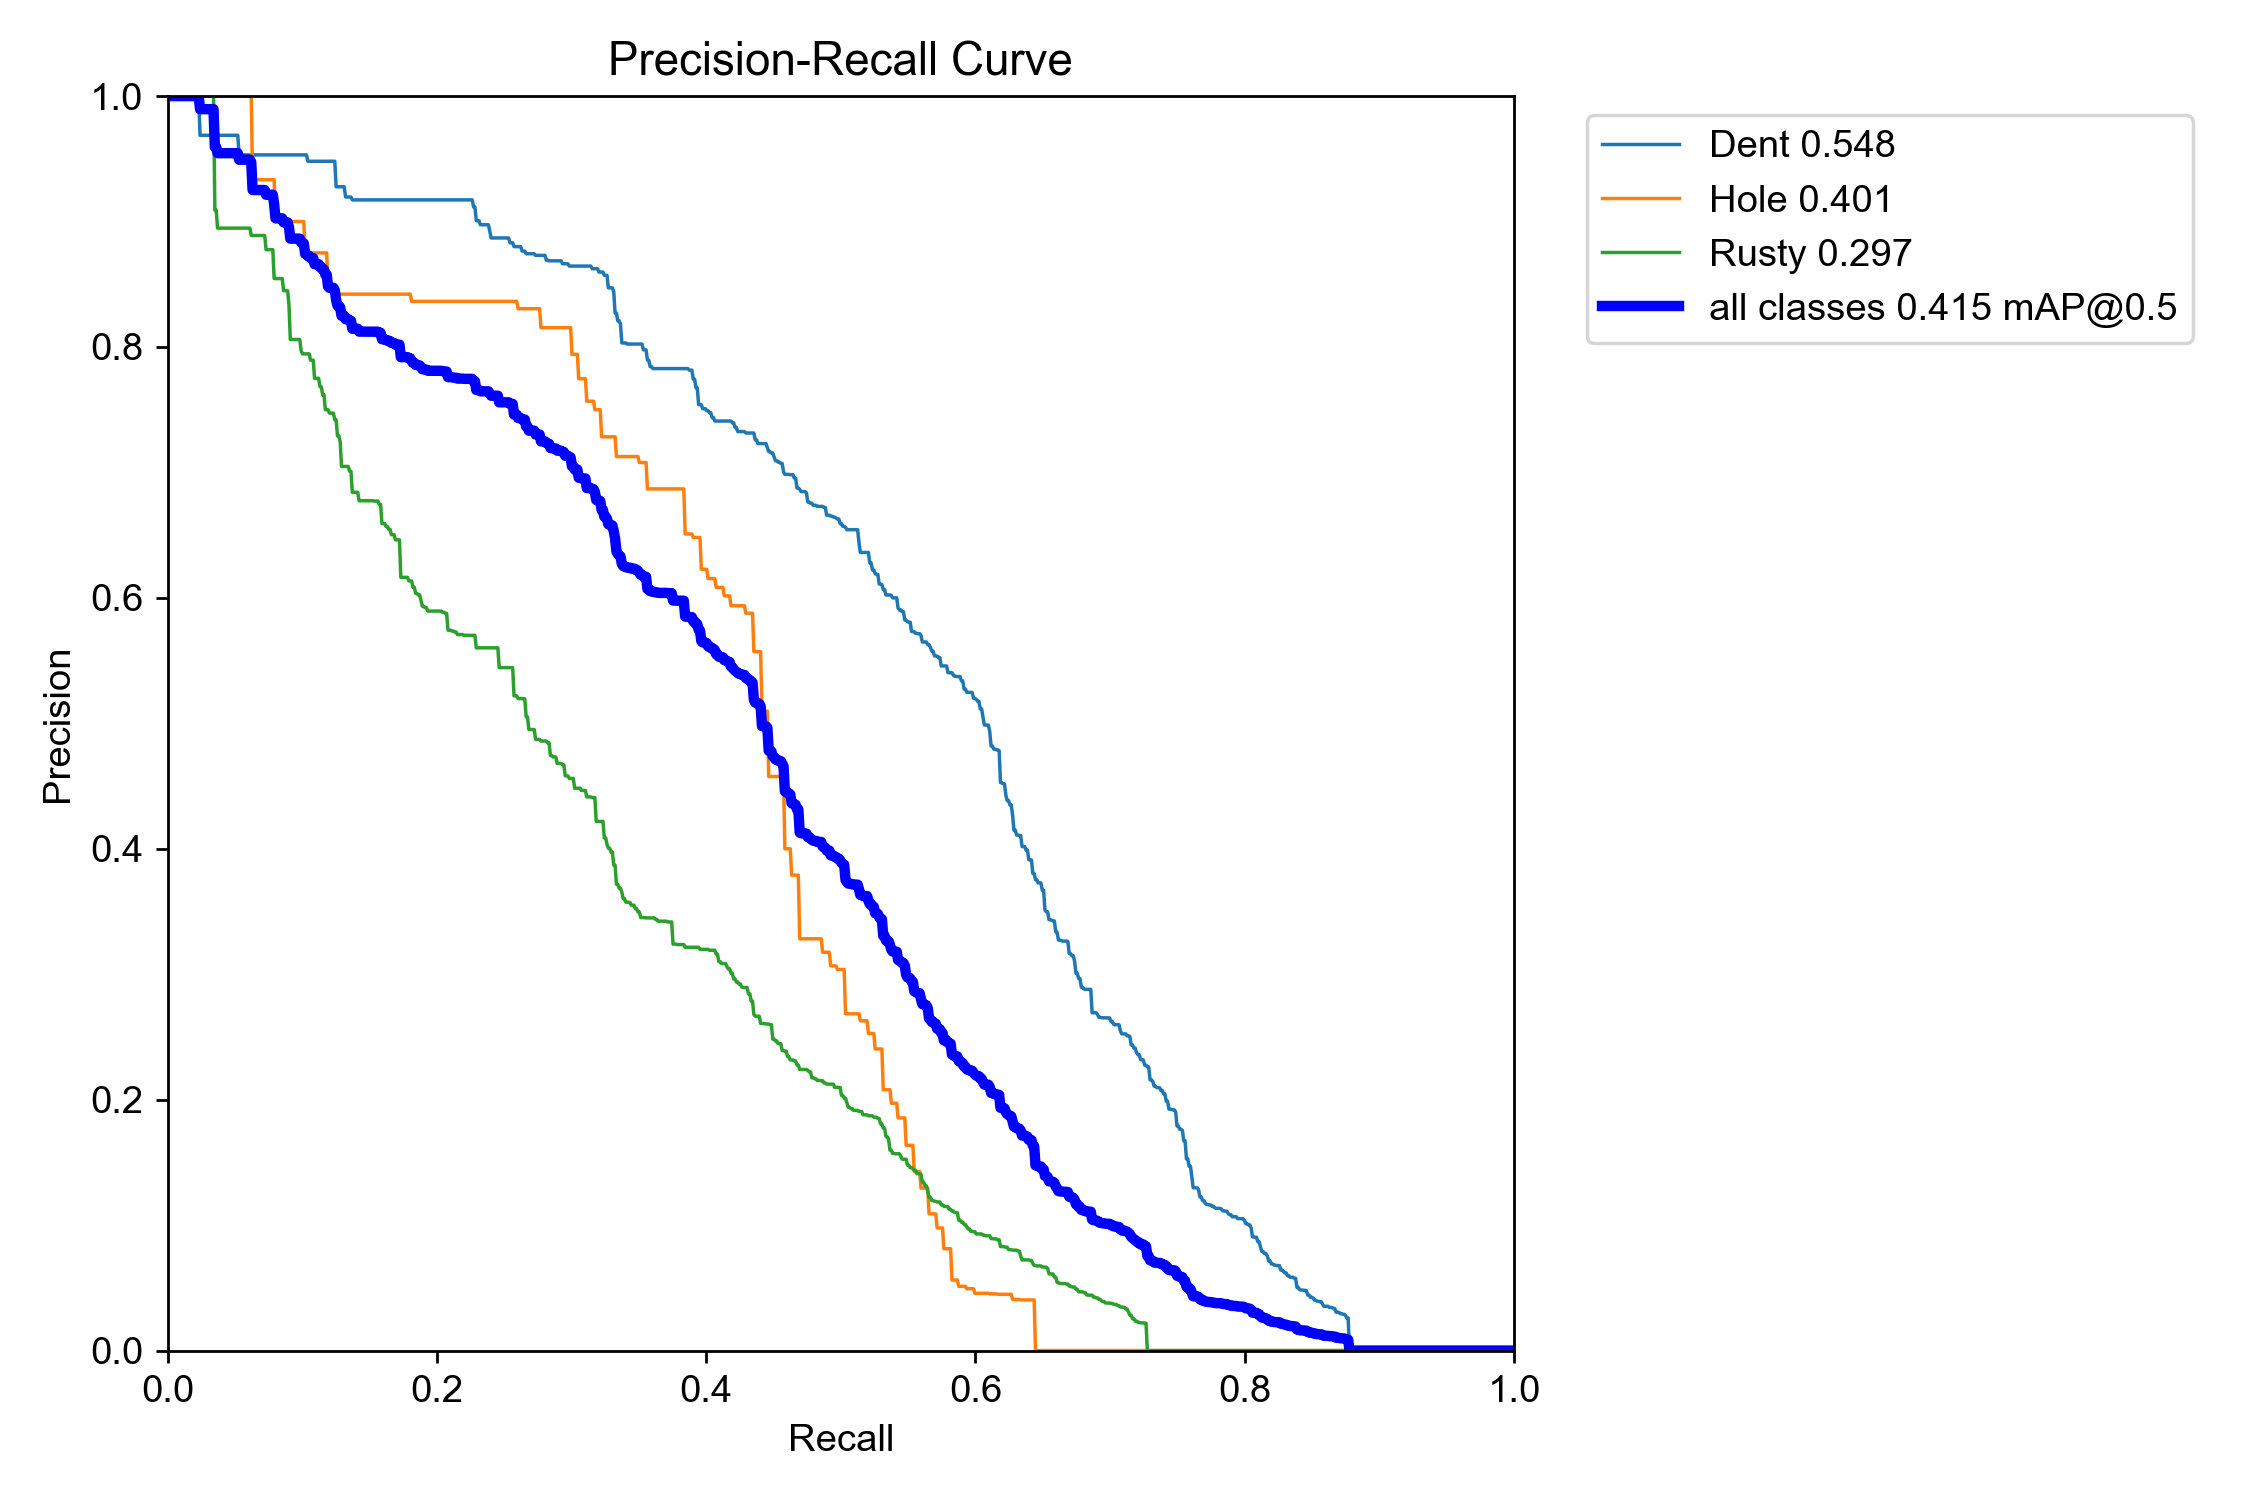
\includegraphics[width=\textwidth]{figures/fig_pr_curve.png}
  \caption{最终模型 PR 曲线}\label{fig:pr}
\end{minipage}
\hfill
\begin{minipage}[t]{0.48\textwidth}
  \centering
  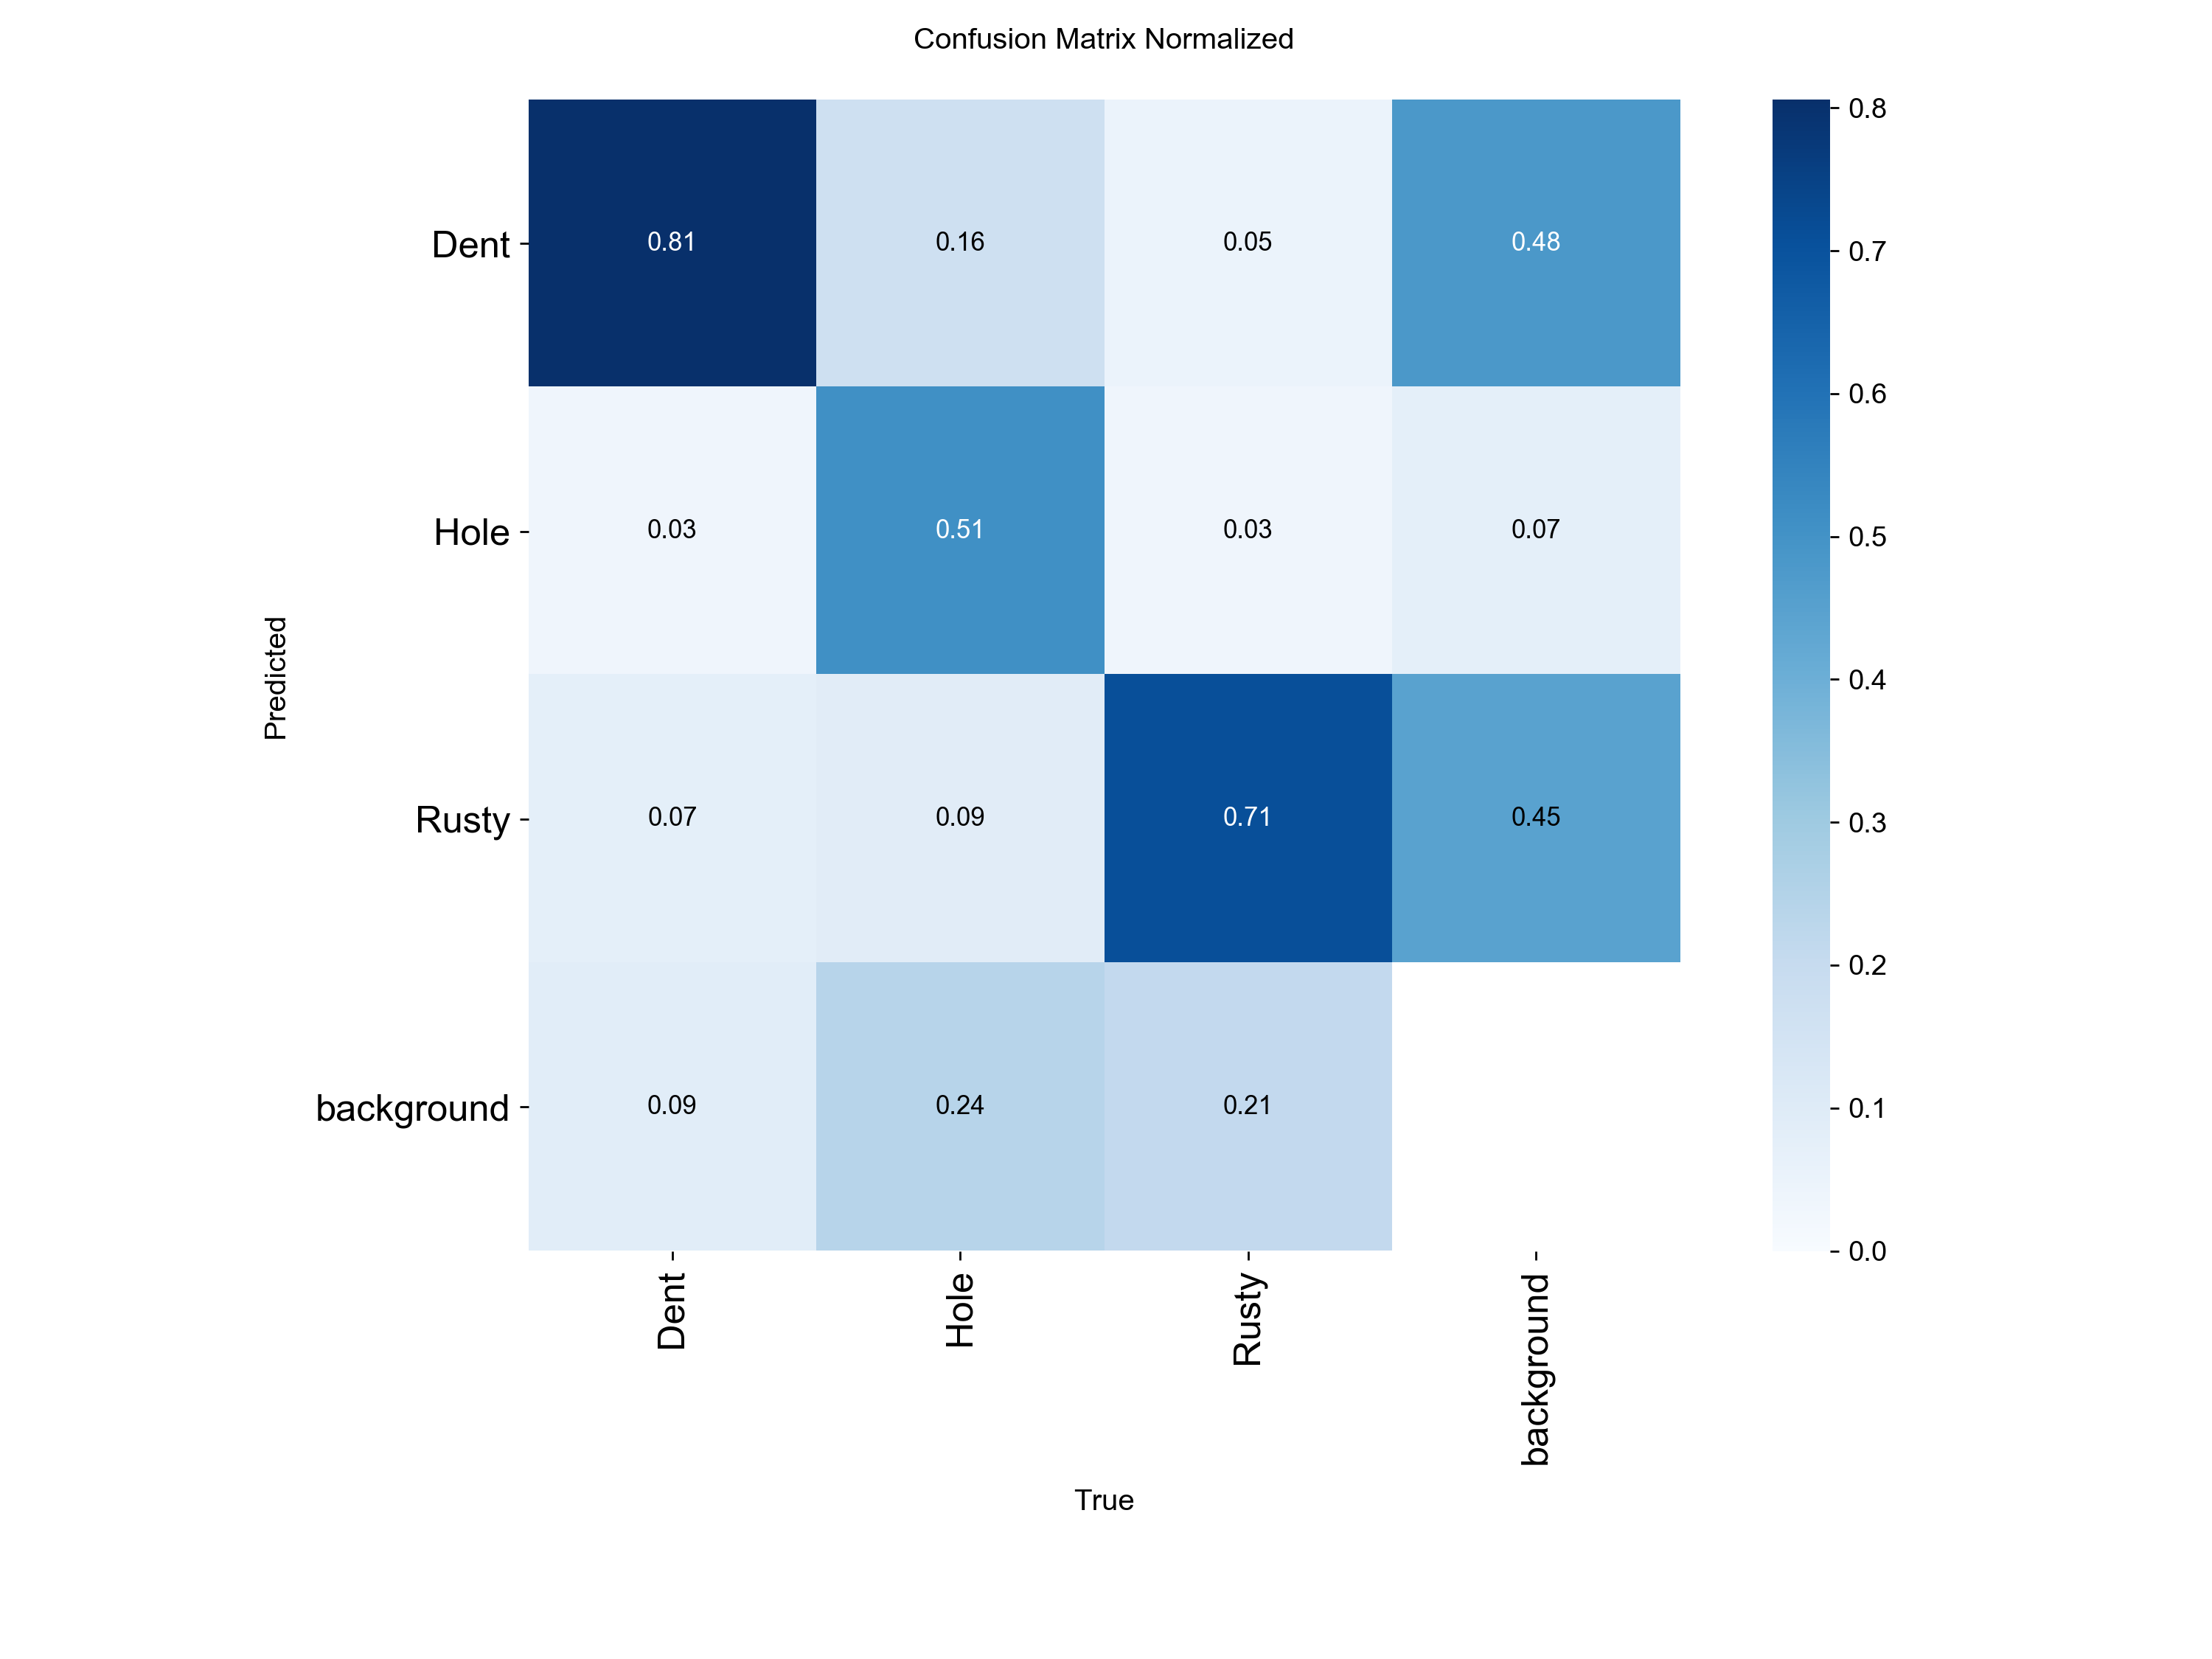
\includegraphics[width=\textwidth]{figures/fig_cm.png}
  \caption{最终模型归一化混淆矩阵}\label{fig:cm}
\end{minipage}
\end{figure}

\begin{figure}[H]
\centering
\begin{minipage}[t]{0.49\textwidth}
  \centering
  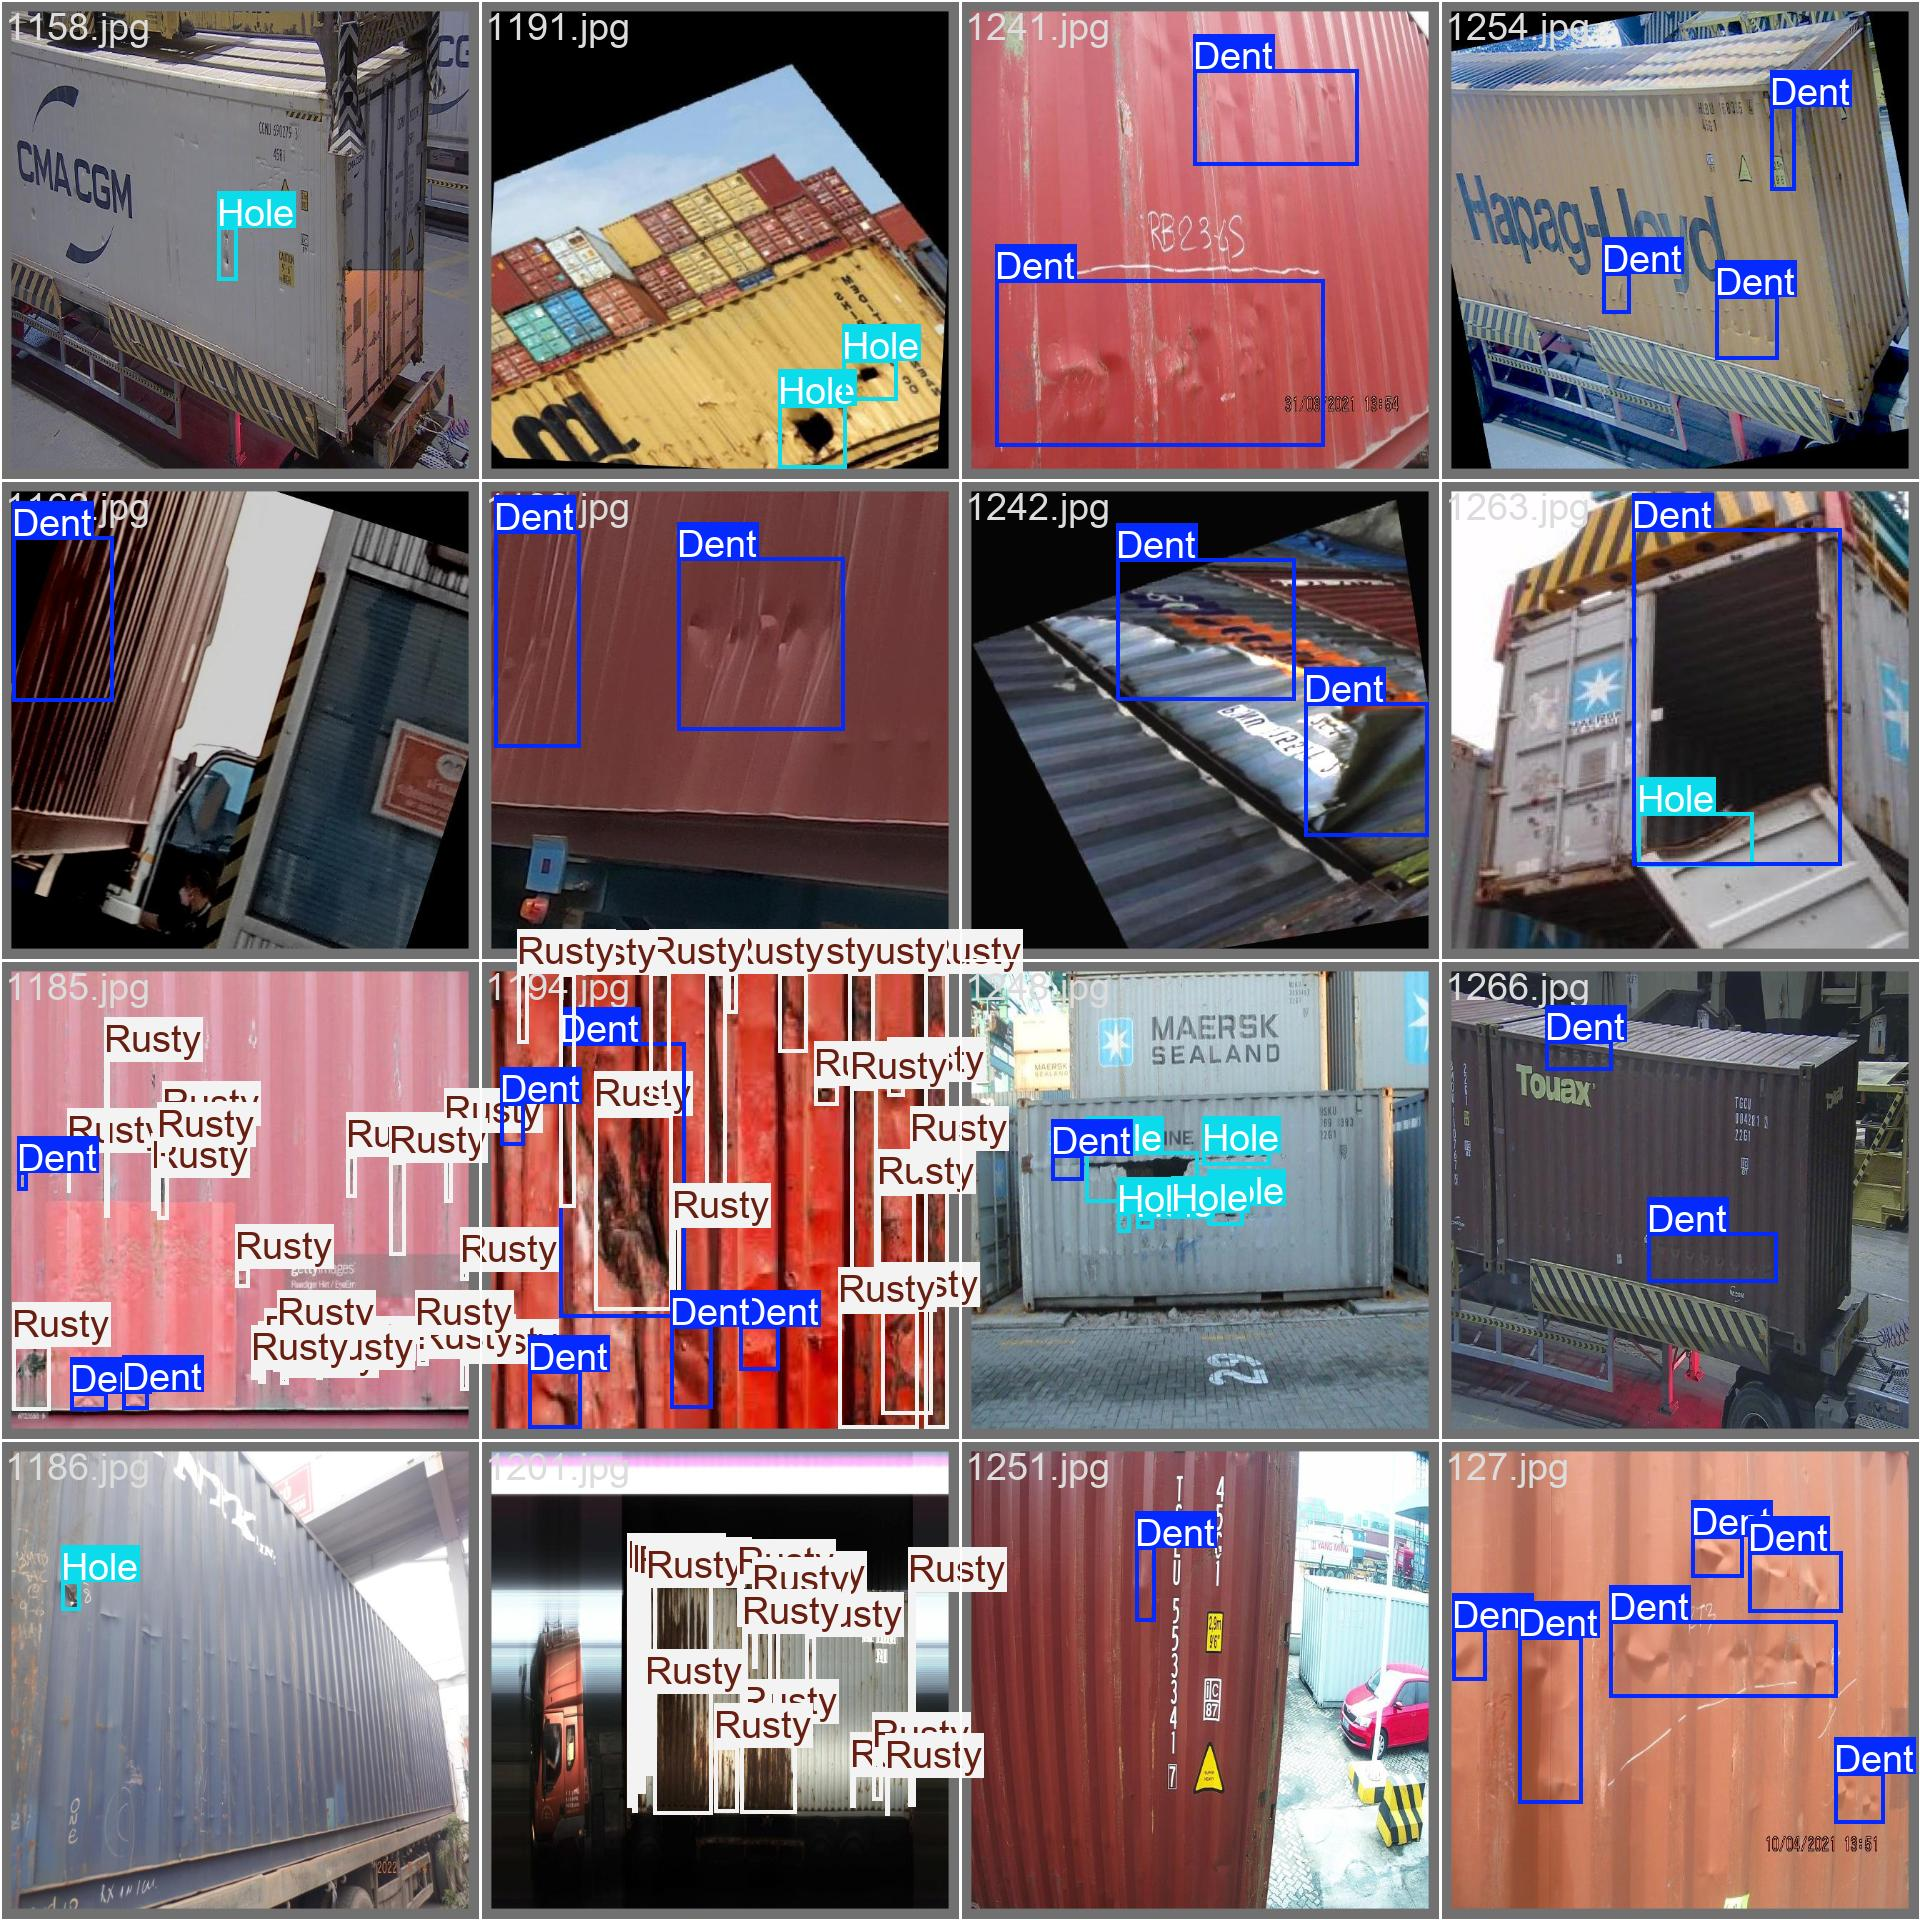
\includegraphics[width=\textwidth]{figures/fig_val_labels.jpg}
  \caption{验证集标注（Ground Truth）}\label{fig:val_labels}
\end{minipage}
\hfill
\begin{minipage}[t]{0.49\textwidth}
  \centering
  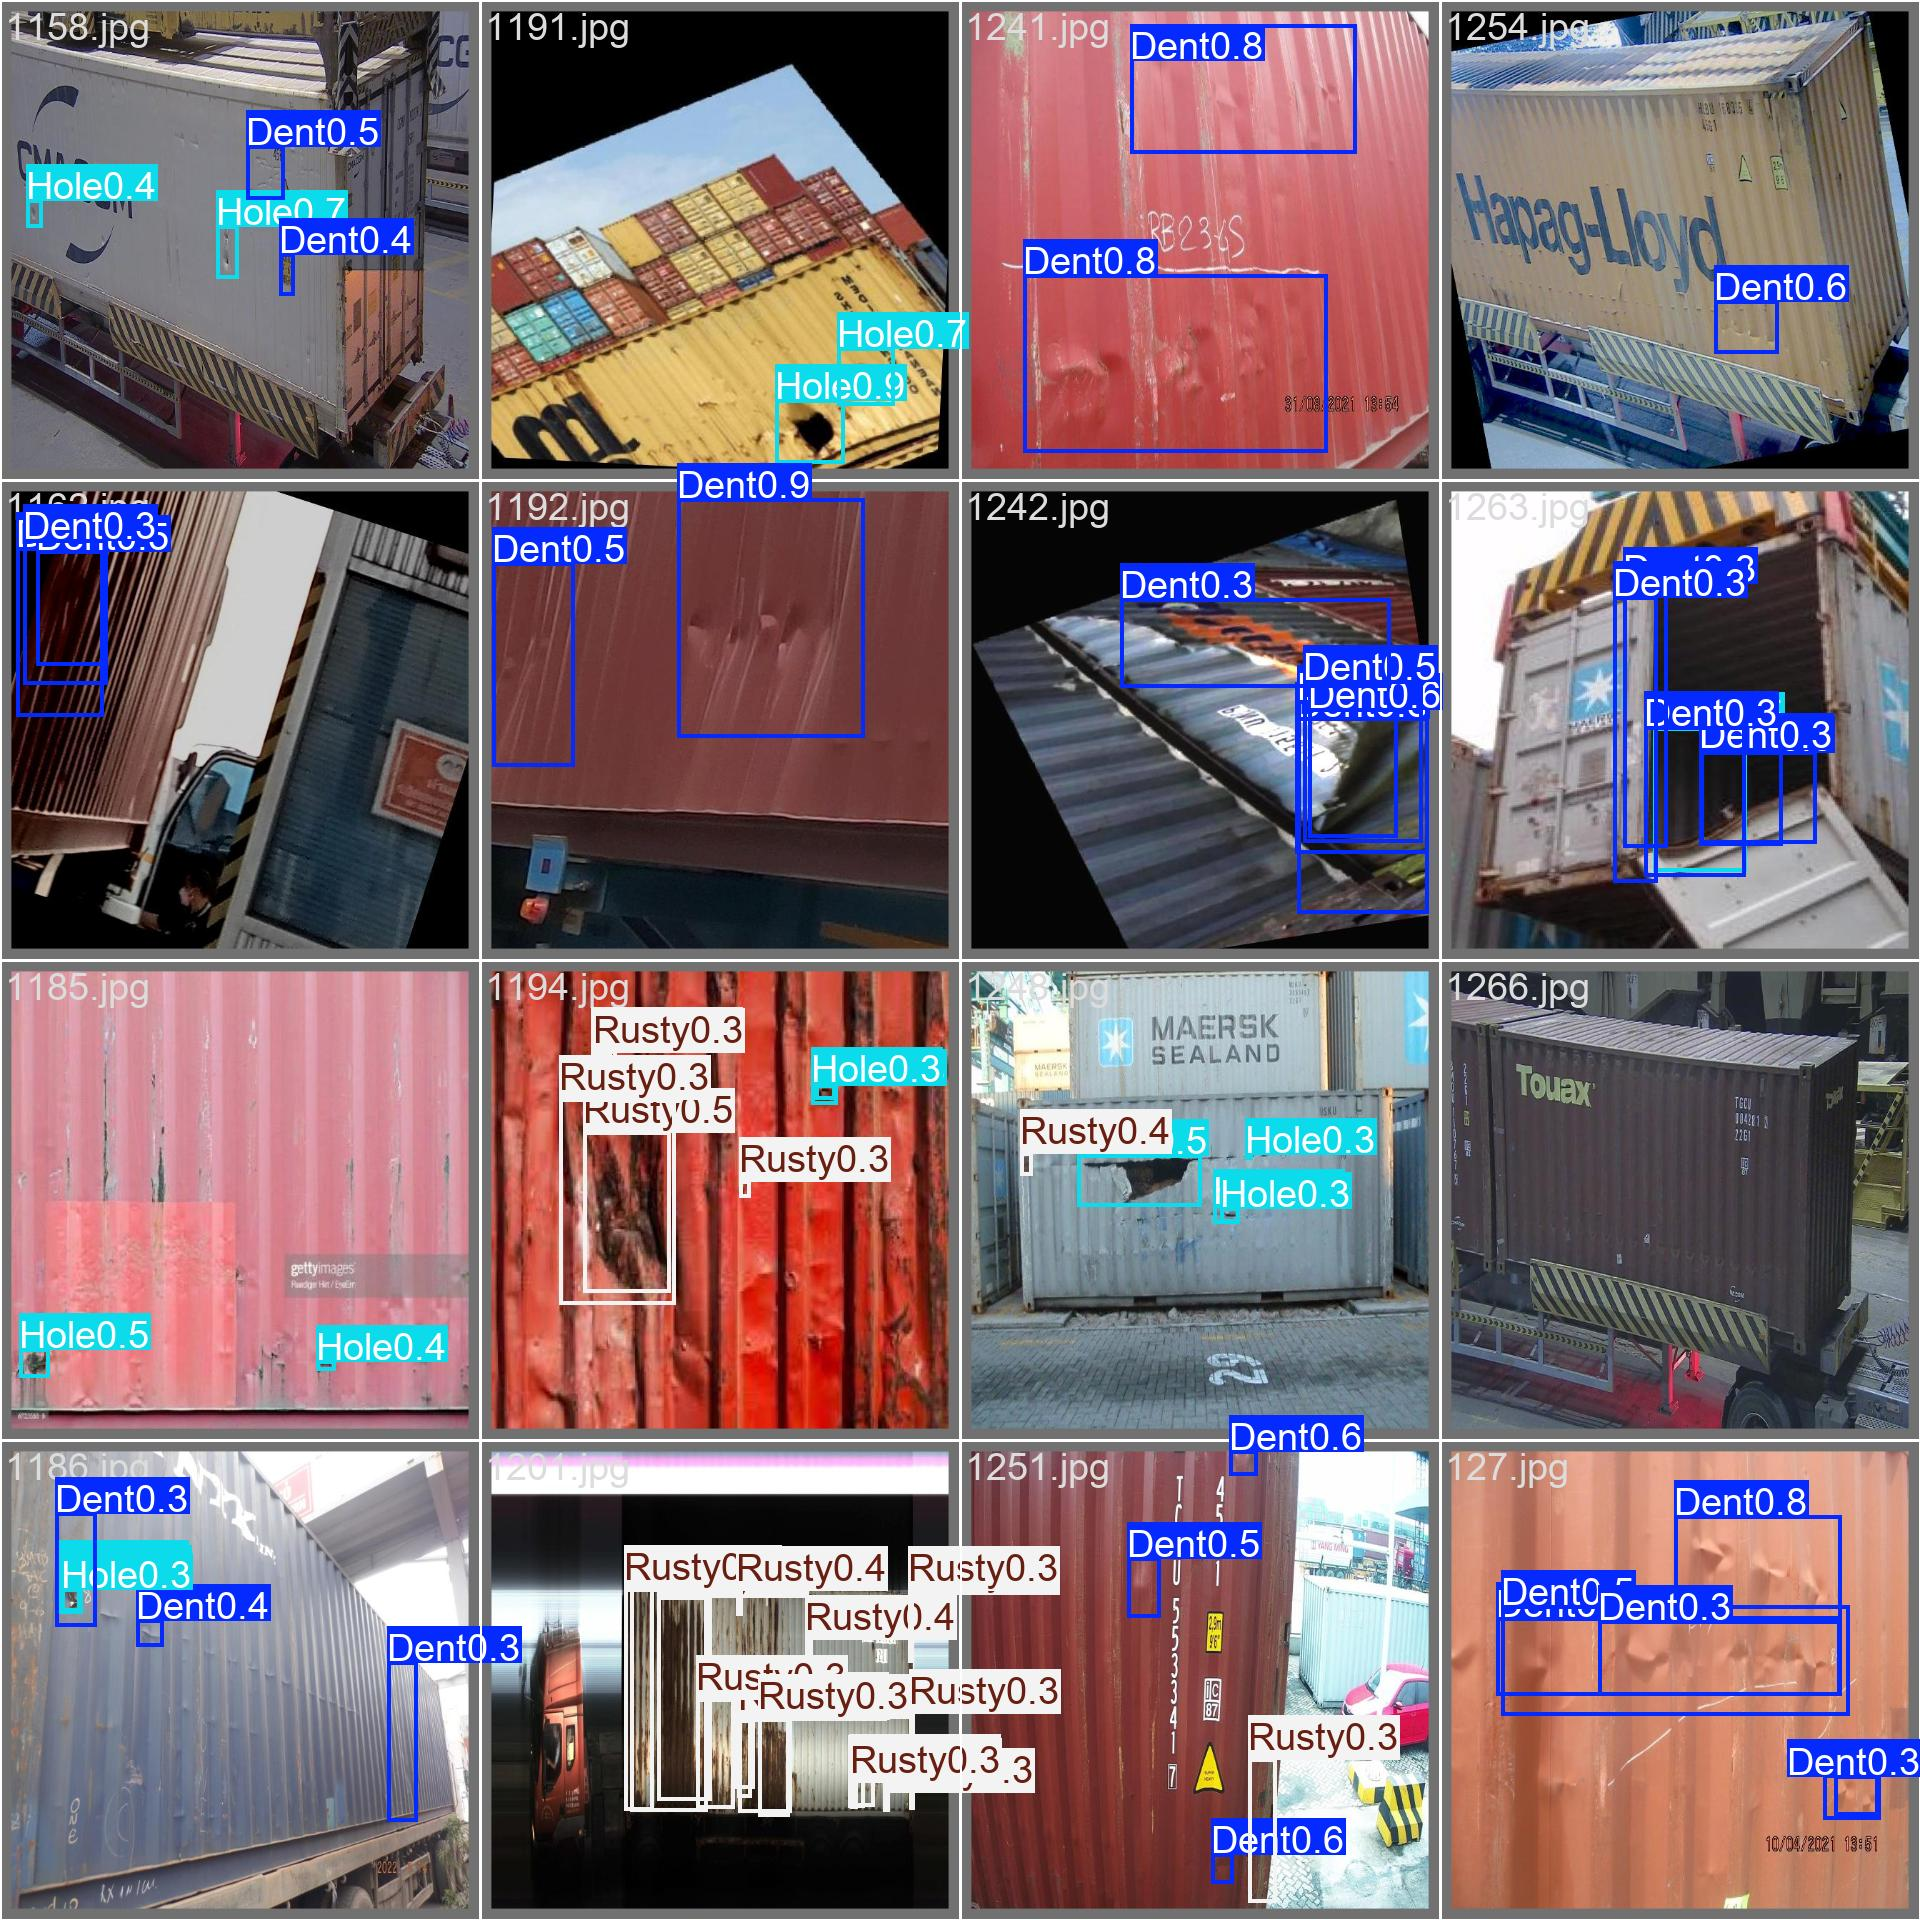
\includegraphics[width=\textwidth]{figures/fig_val_pred.jpg}
  \caption{验证集模型预测}\label{fig:val_pred}
\end{minipage}
\end{figure}

\begin{figure}[H]
\centering
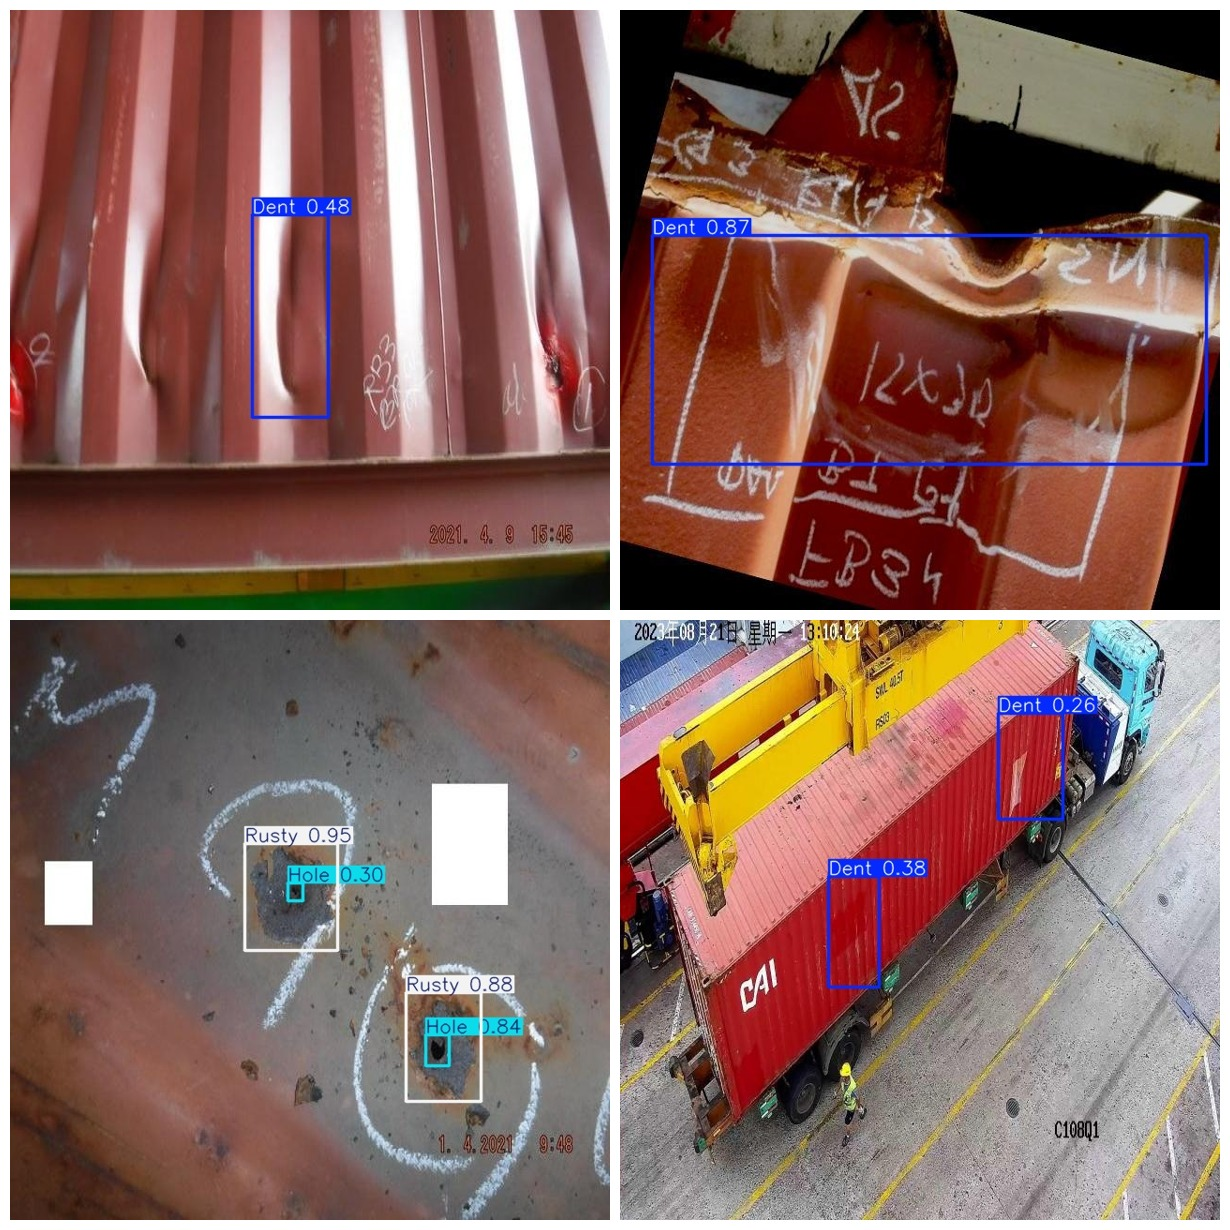
\includegraphics[width=0.96\textwidth]{figures/fig_detect_results.jpg}
\caption{测试集检测结果可视化示例}\label{fig:detect_samples}
\end{figure}

\subsubsection{检测结果提交}

利用最终模型对 413 幅测试图像进行推理（置信度阈值 0.25，NMS 阈值 0.45），检测结果按六列格式（\texttt{image\_id}、\texttt{class\_id}、\texttt{x\_center}、\texttt{y\_center}、\texttt{width}、\texttt{height}）写入 \texttt{test\_result.csv}。共输出 931 个检测框，覆盖 377 幅图像（其余 36 幅无检测框），各类别数量如表 \ref{tab:submit} 所示，类别比例与训练集分布基本一致。

\begin{table}[H]
\centering
\zihao{5}
\caption{test\_result.csv 提交检测结果统计}\label{tab:submit}
\begin{tabular}{lcc}
  \toprule
  类别 & 检测框数 & 占比 \\
  \midrule
  Dent（凹陷） & 463 & 49.7\% \\
  Hole（破洞） & 131 & 14.1\% \\
  Rusty（锈蚀） & 337 & 36.2\% \\
  \midrule
  合计 & 931 & 100.0\% \\
  \bottomrule
\end{tabular}
\end{table}
